\documentclass{article}
\usepackage[utf8]{inputenc}
\usepackage[spanish]{babel}
\usepackage{listings}
\usepackage{subfigure}
\usepackage{graphicx}
\usepackage{url}
\usepackage{multirow}
\usepackage{color}
\usepackage{booktabs}
\usepackage{float}

\usepackage{hyperref}
\usepackage[margin=3cm,twoside]{geometry} 
\setlength{\parindent}{0pt}
\setlength{\parskip}{1em}


\definecolor{mygreen}{rgb}{0,0.6,0}
\definecolor{mygray}{rgb}{0.5,0.5,0.5}
\definecolor{mymauve}{rgb}{0.58,0,0.82}
\lstset{ 
  backgroundcolor=\color{white},   % choose the background color; you must add \usepackage{color} or \usepackage{xcolor}; should come as last argument
  basicstyle=\footnotesize,        % the size of the fonts that are used for the code
  breakatwhitespace=false,         % sets if automatic breaks should only happen at whitespace
  breaklines=true,                 % sets automatic line breaking
  captionpos=b,                    % sets the caption-position to bottom
  commentstyle=\color{mygreen},    % comment style
  deletekeywords={...},            % if you want to delete keywords from the given language
  escapeinside={\%}{)},          % if you want to add LaTeX within your code
  extendedchars=true,              % lets you use non-ASCII characters; for 8-bits encodings only, does not work with UTF-8
  firstnumber=1,                % start line enumeration with line 1000
  frame=single,	                   % adds a frame around the code
  keepspaces=true,                 % keeps spaces in text, useful for keeping indentation of code (possibly needs columns=flexible)
  keywordstyle=\color{blue},       % keyword style
  language=Octave,                 % the language of the code
  morekeywords={*,...},            % if you want to add more keywords to the set
  numbers=left,                    % where to put the line-numbers; possible values are (none, left, right)
  numbersep=5pt,                   % how far the line-numbers are from the code
  numberstyle=\tiny\color{mygray}, % the style that is used for the line-numbers
  rulecolor=\color{black},         % if not set, the frame-color may be changed on line-breaks within not-black text (e.g. comments (green here))
  showspaces=false,                % show spaces everywhere adding particular underscores; it overrides 'showstringspaces'
  showstringspaces=false,          % underline spaces within strings only
  showtabs=false,                  % show tabs within strings adding particular underscores
  stepnumber=1,                    % the step between two line-numbers. If it's 1, each line will be numbered
  stringstyle=\color{mymauve},     % string literal style
  tabsize=2,	                   % sets default tabsize to 2 spaces
  title=\lstname                  % show the filename of files included with \lstinputlisting; also try caption instead of title
}
\usepackage{etoolbox}
\makeatletter
\providecommand{\subtitle}[1]{% add subtitle to \maketitle
  \apptocmd{\@title}{\par {\large #1 \par}}{}{}
}
\makeatother
\title{Tarea 4 de Modelos Probabilistas Aplicados}
\subtitle{Distribución de Poisson}

\author{5271}
\date{\today}

\begin{document}

\maketitle

\section{Introducción}

En este trabajo se presenta un acercamiento a la simulación de variables aleatorias de Poisson a partir de variables aleatorias de distribución Uniforme, Exponencial y Normal. Además se presenta la aproximación de la distribución de Poisson a la distribución Binomial que seguían los largos de palabras de libro ``The Adventures of Sherlock Holmes" \cite{Holmes92}. Este libro se encuentra disponible en la biblioteca virtual gratuita Project Gutenberg, con el siguiente enlace: \href{https://www.gutenberg.org}{https://www.gutenberg.org}. 

\section{Proceso de Poisson}

La distribución de Poisson es una distribución de probabilidad discreta que expresa, a partir de una frecuencia de ocurrencia media, la probabilidad de que ocurra un determinado número de eventos durante cierto período de tiempo o espacio. Se centra en la probabilidad de ocurrencia de eventos con probabilidades muy pequeñas. Se especifica por un parámetro lambda $(\lambda)$. Este parámetro es igual a la media y la varianza de la distribución. 

\section{Aproximación mediante el uso de variables aleatorias Exponenciales }

Los momentos en que se incrementa el proceso de Poisson se denominan tiempos de llegada o tiempos de ocurrencia , ya que en los modelos estocásticos clásicos representan las llegadas o ocurrencias de algo, como llegadas de clientes a la fila de un banco. Las diferencias entre tiempos consecutivos se denominan tiempos entre llegadas. Los tiempos entre llegadas de un proceso de Poisson homogéneo lo forman variables aleatorias exponenciales independientes , un resultado conocido como el Teorema del intervalo . A partir de esta relación se pueden generar variables aleatorias exponenciales $E_{1}, E_{2},...N_{n}$ y N es el número entero más pequeño tal que:

\begin{equation}
    \sum_{k=1}^{n}E_{k}>1 
\end{equation}
Entonces N es Poisson $(\lambda)$, Lema 3.2 Capítulo 10 \cite{expvar}  

A continuación realizaremos una comparación entre las variables aleatorias de Poisson creadas a partir de la suma de las variables aleatorias exponenciales y las creadas a partir de la biblioteca \textit{rpois}.

En la figura \ref{fig:1} de la página \pageref{fig:1} se muestra los histogramas de las dos poblaciones simuladas. En la figura \ref{fig:2} de la página \pageref{fig:2}, se muestran superpuestos los diagramas de densidad de ambas poblaciones 

\begin{center}
\begin{figure}
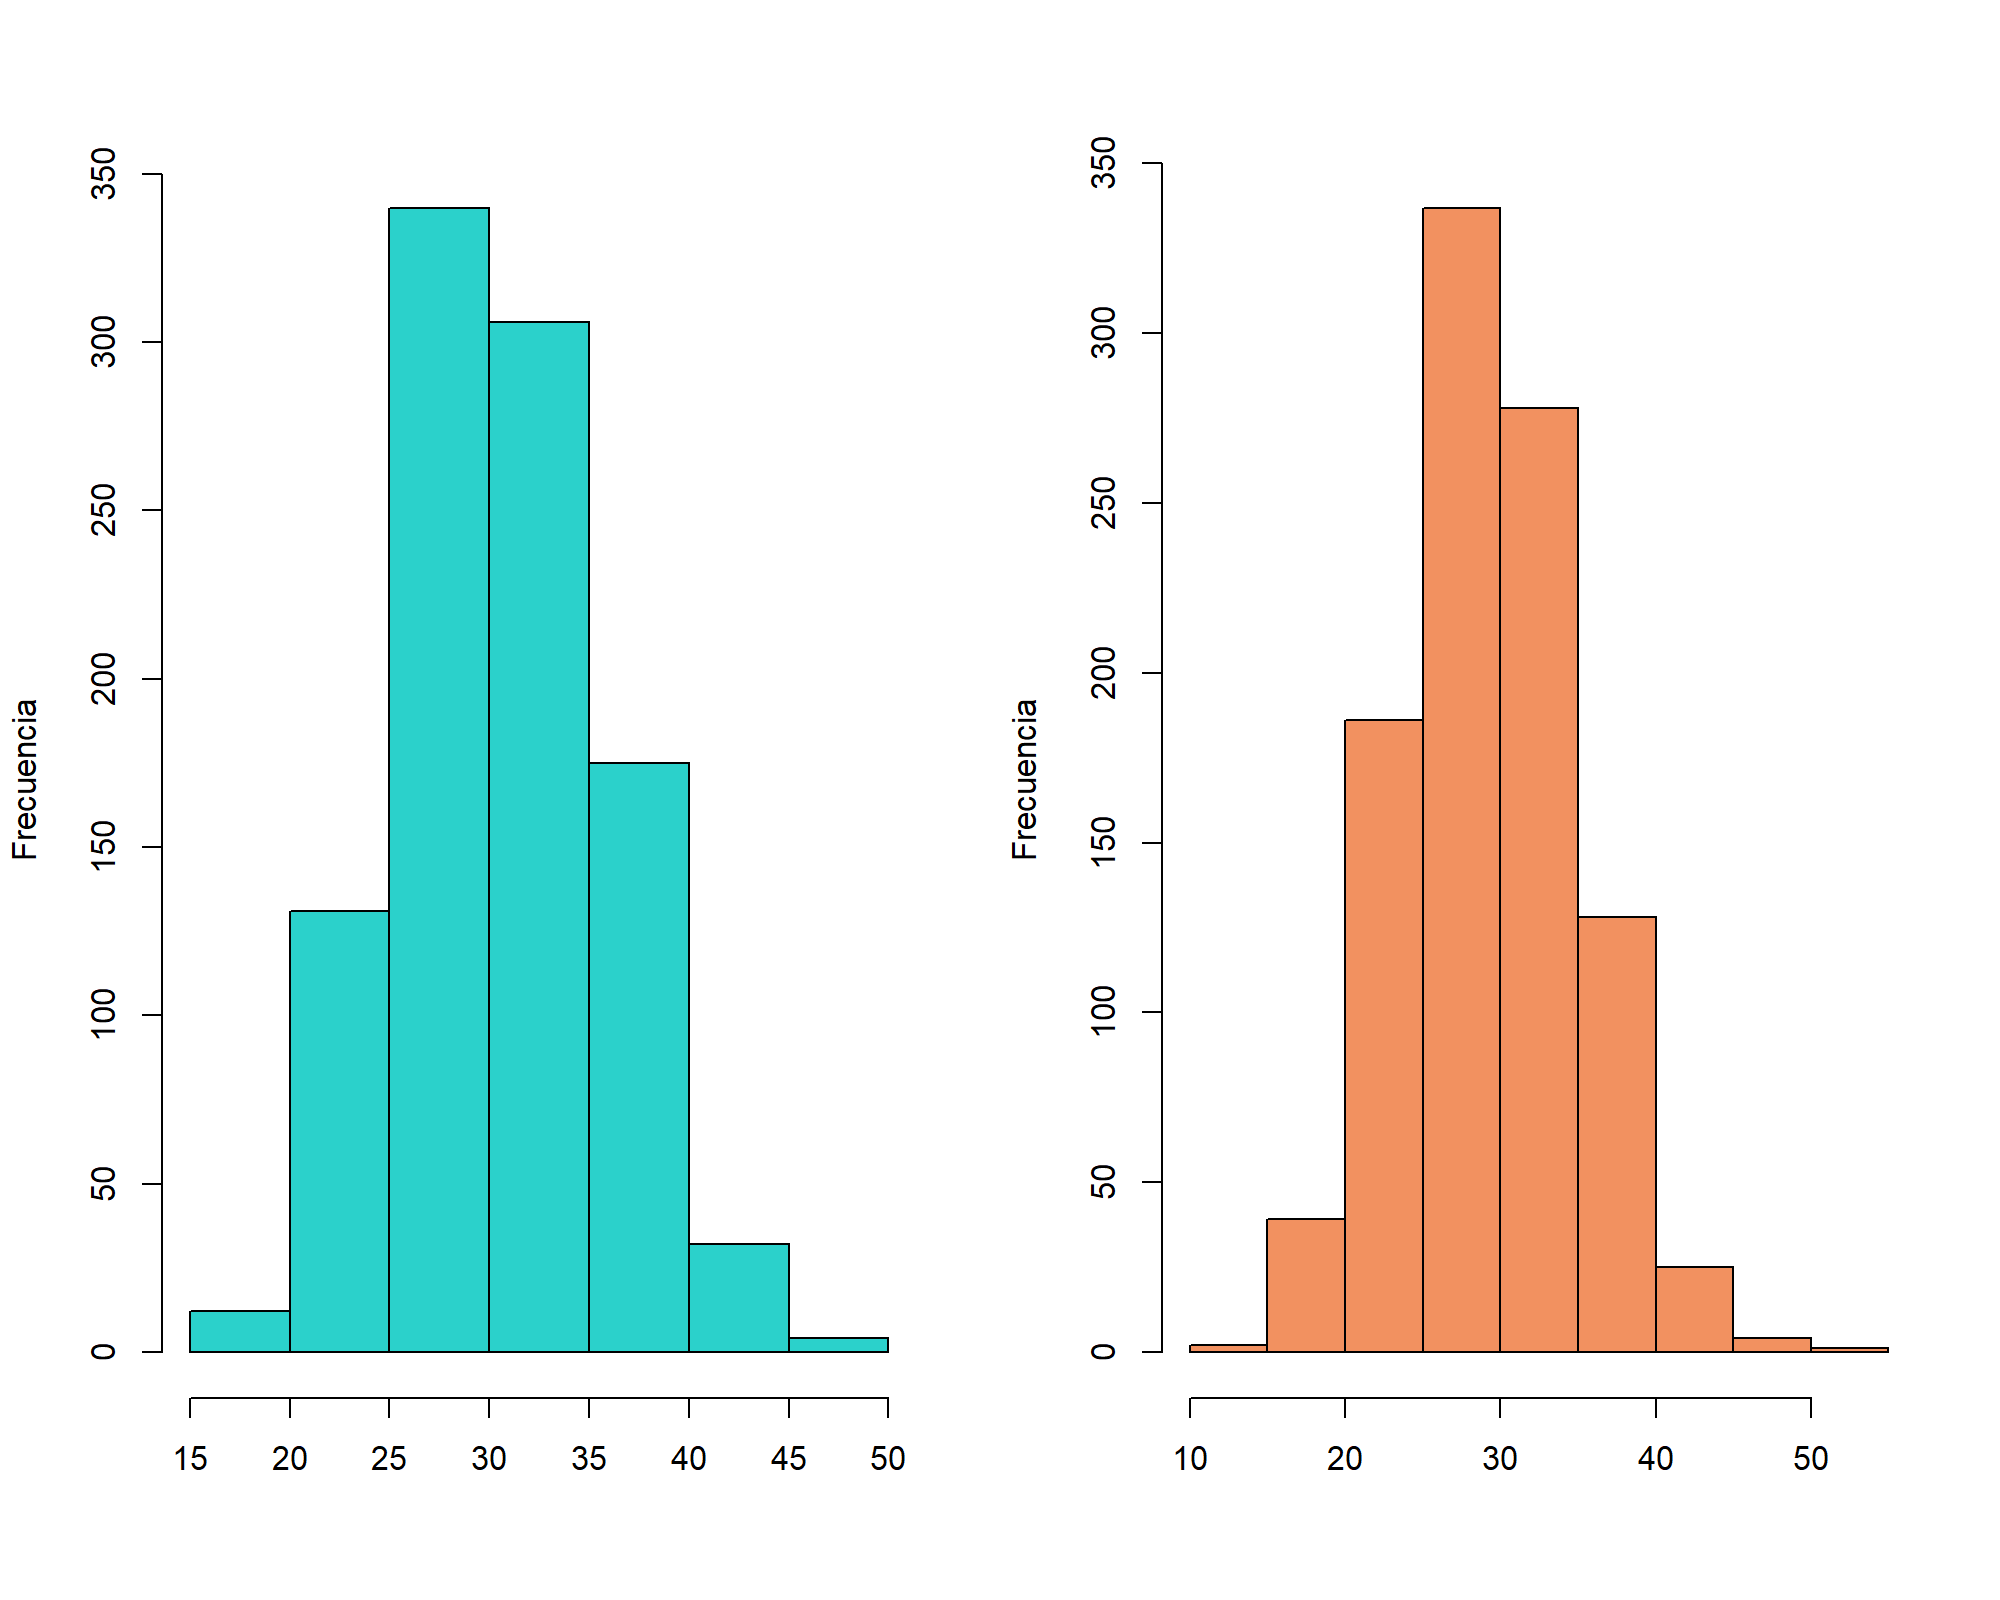
\includegraphics[scale=0.65]{figuras/AproxEx30.png}
\caption{Histogramas de las poblaciones simuladas, a la izquierda la aproximación a partir de la exponencial y a la derecha la creada a partir de la biblioteca \textit{rpois}}
\label{fig:1}
\end{figure}
\end{center}

\begin{center}
\begin{figure}
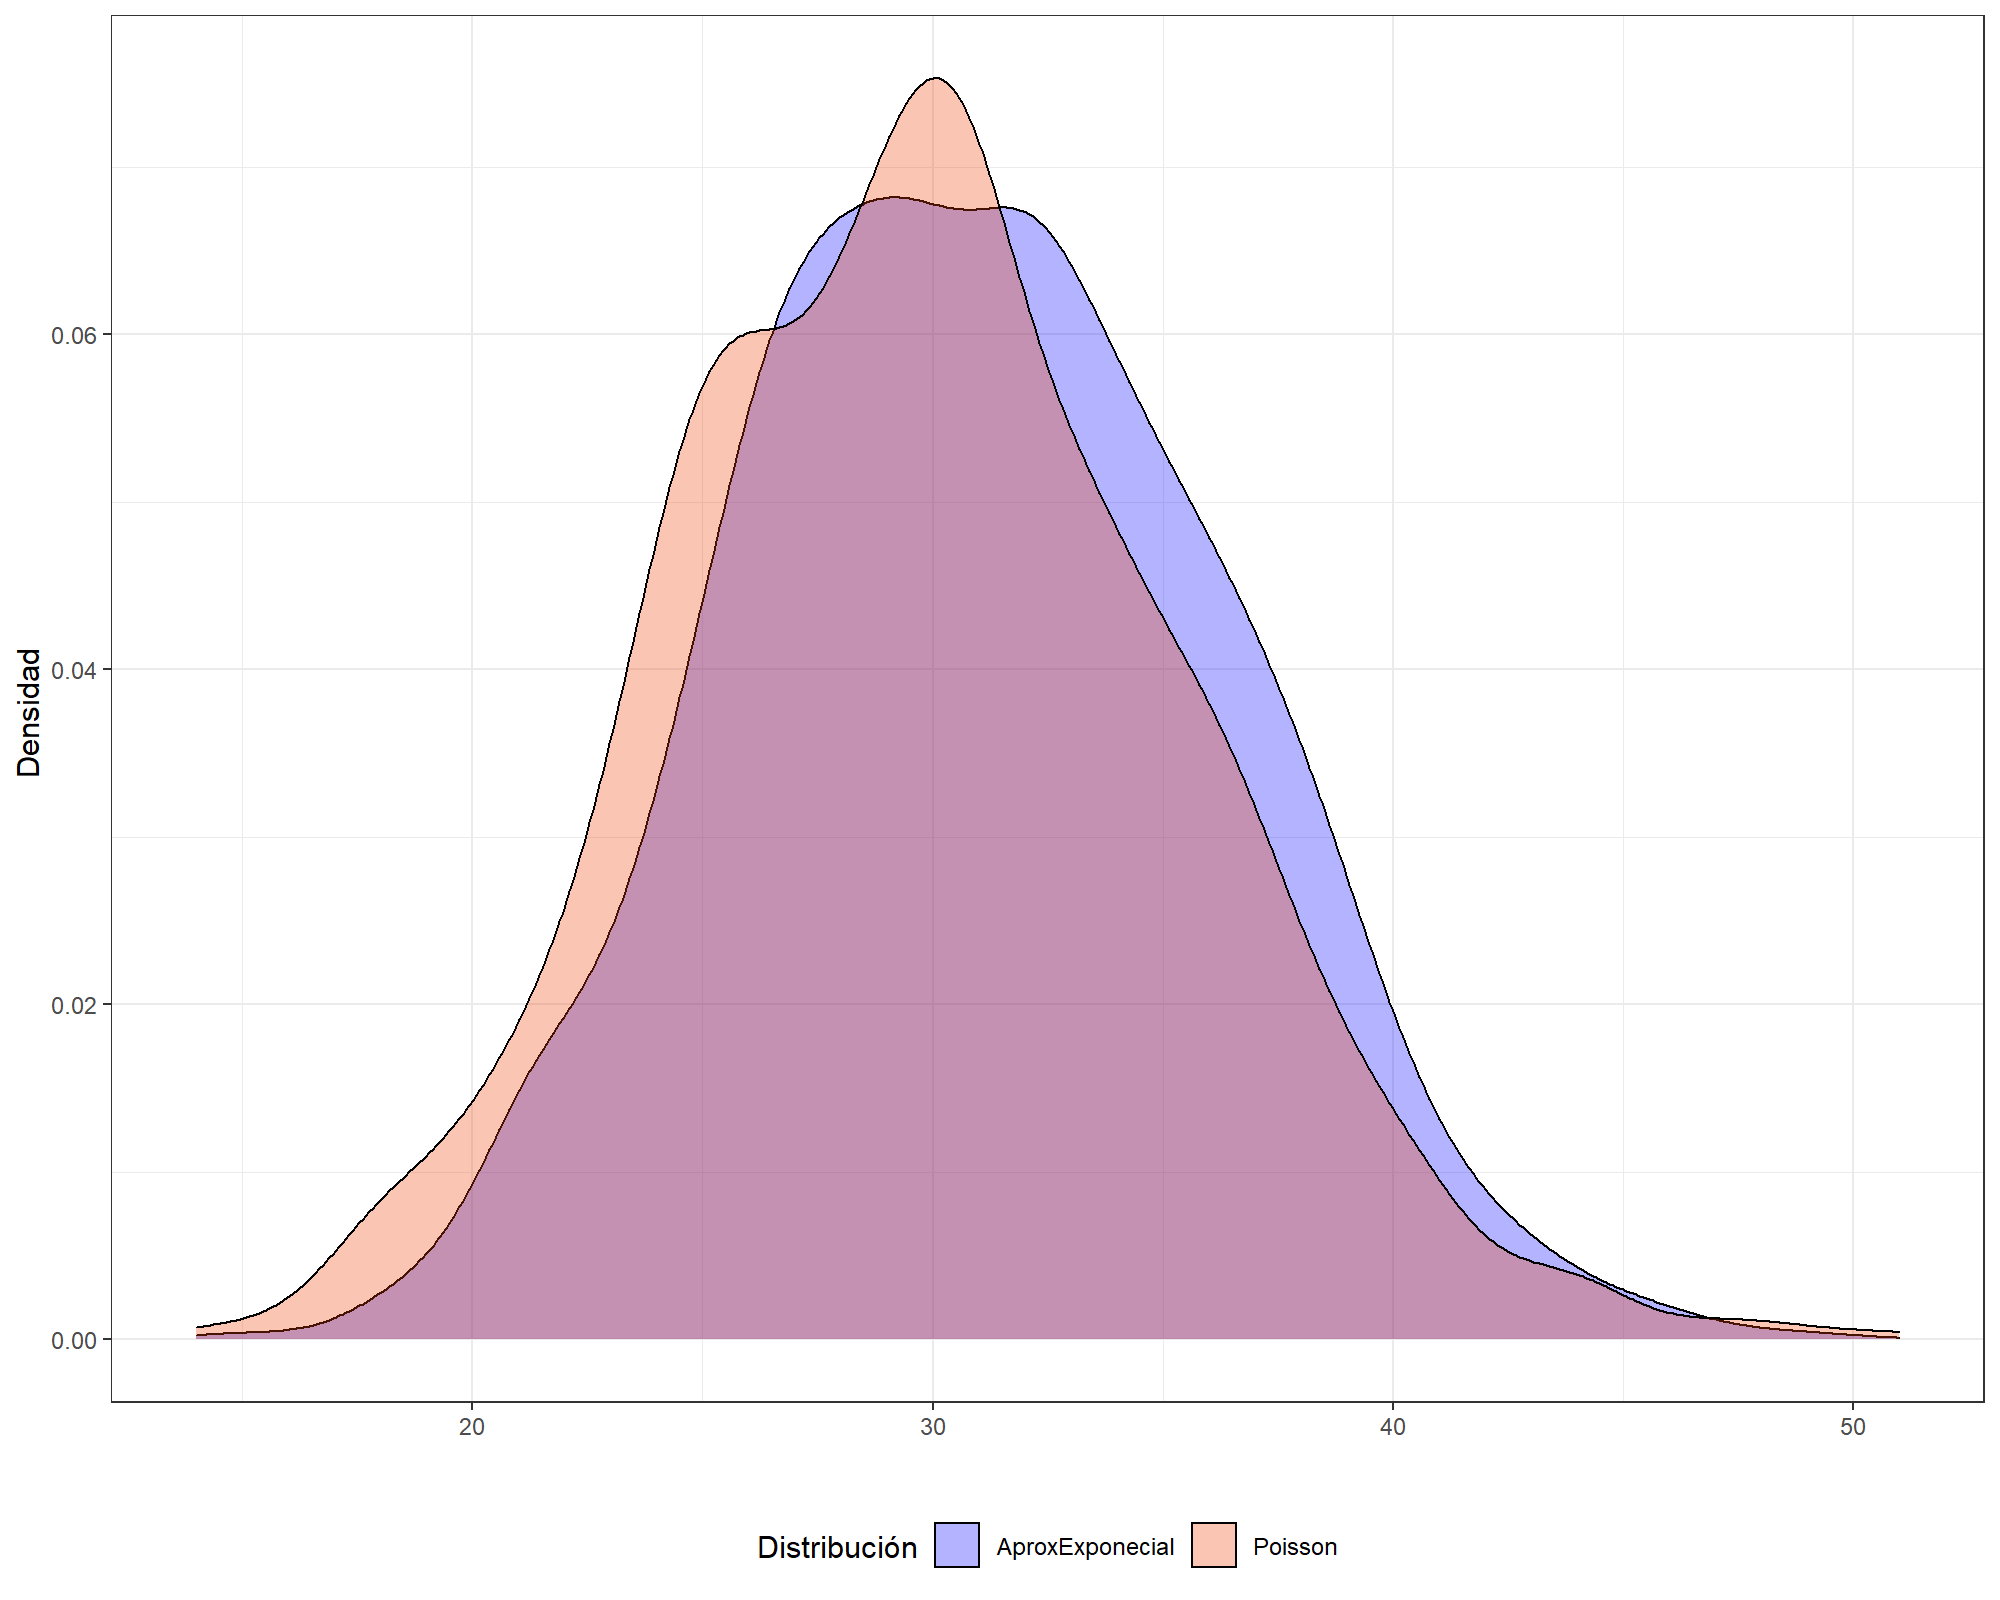
\includegraphics[scale=0.6]{figuras/densidadPE.png}
\caption{Diagramas de densidad de ambas poblaciones}
\label{fig:2}
\end{figure}
\end{center}
Para calcular la diferencia entre las distribuciones se realiza el cálculo de la distancia Kolmogorov–--Smirnov, que se define como la distancia vertical máxima entre las funciones de distribución acumulada empíricas de dos muestras, donde el valor de la distancia es $0.11$. Esto se puede observar en la figura \ref{fig:3} de la página \pageref{fig:3}.

\begin{center}
\begin{figure}
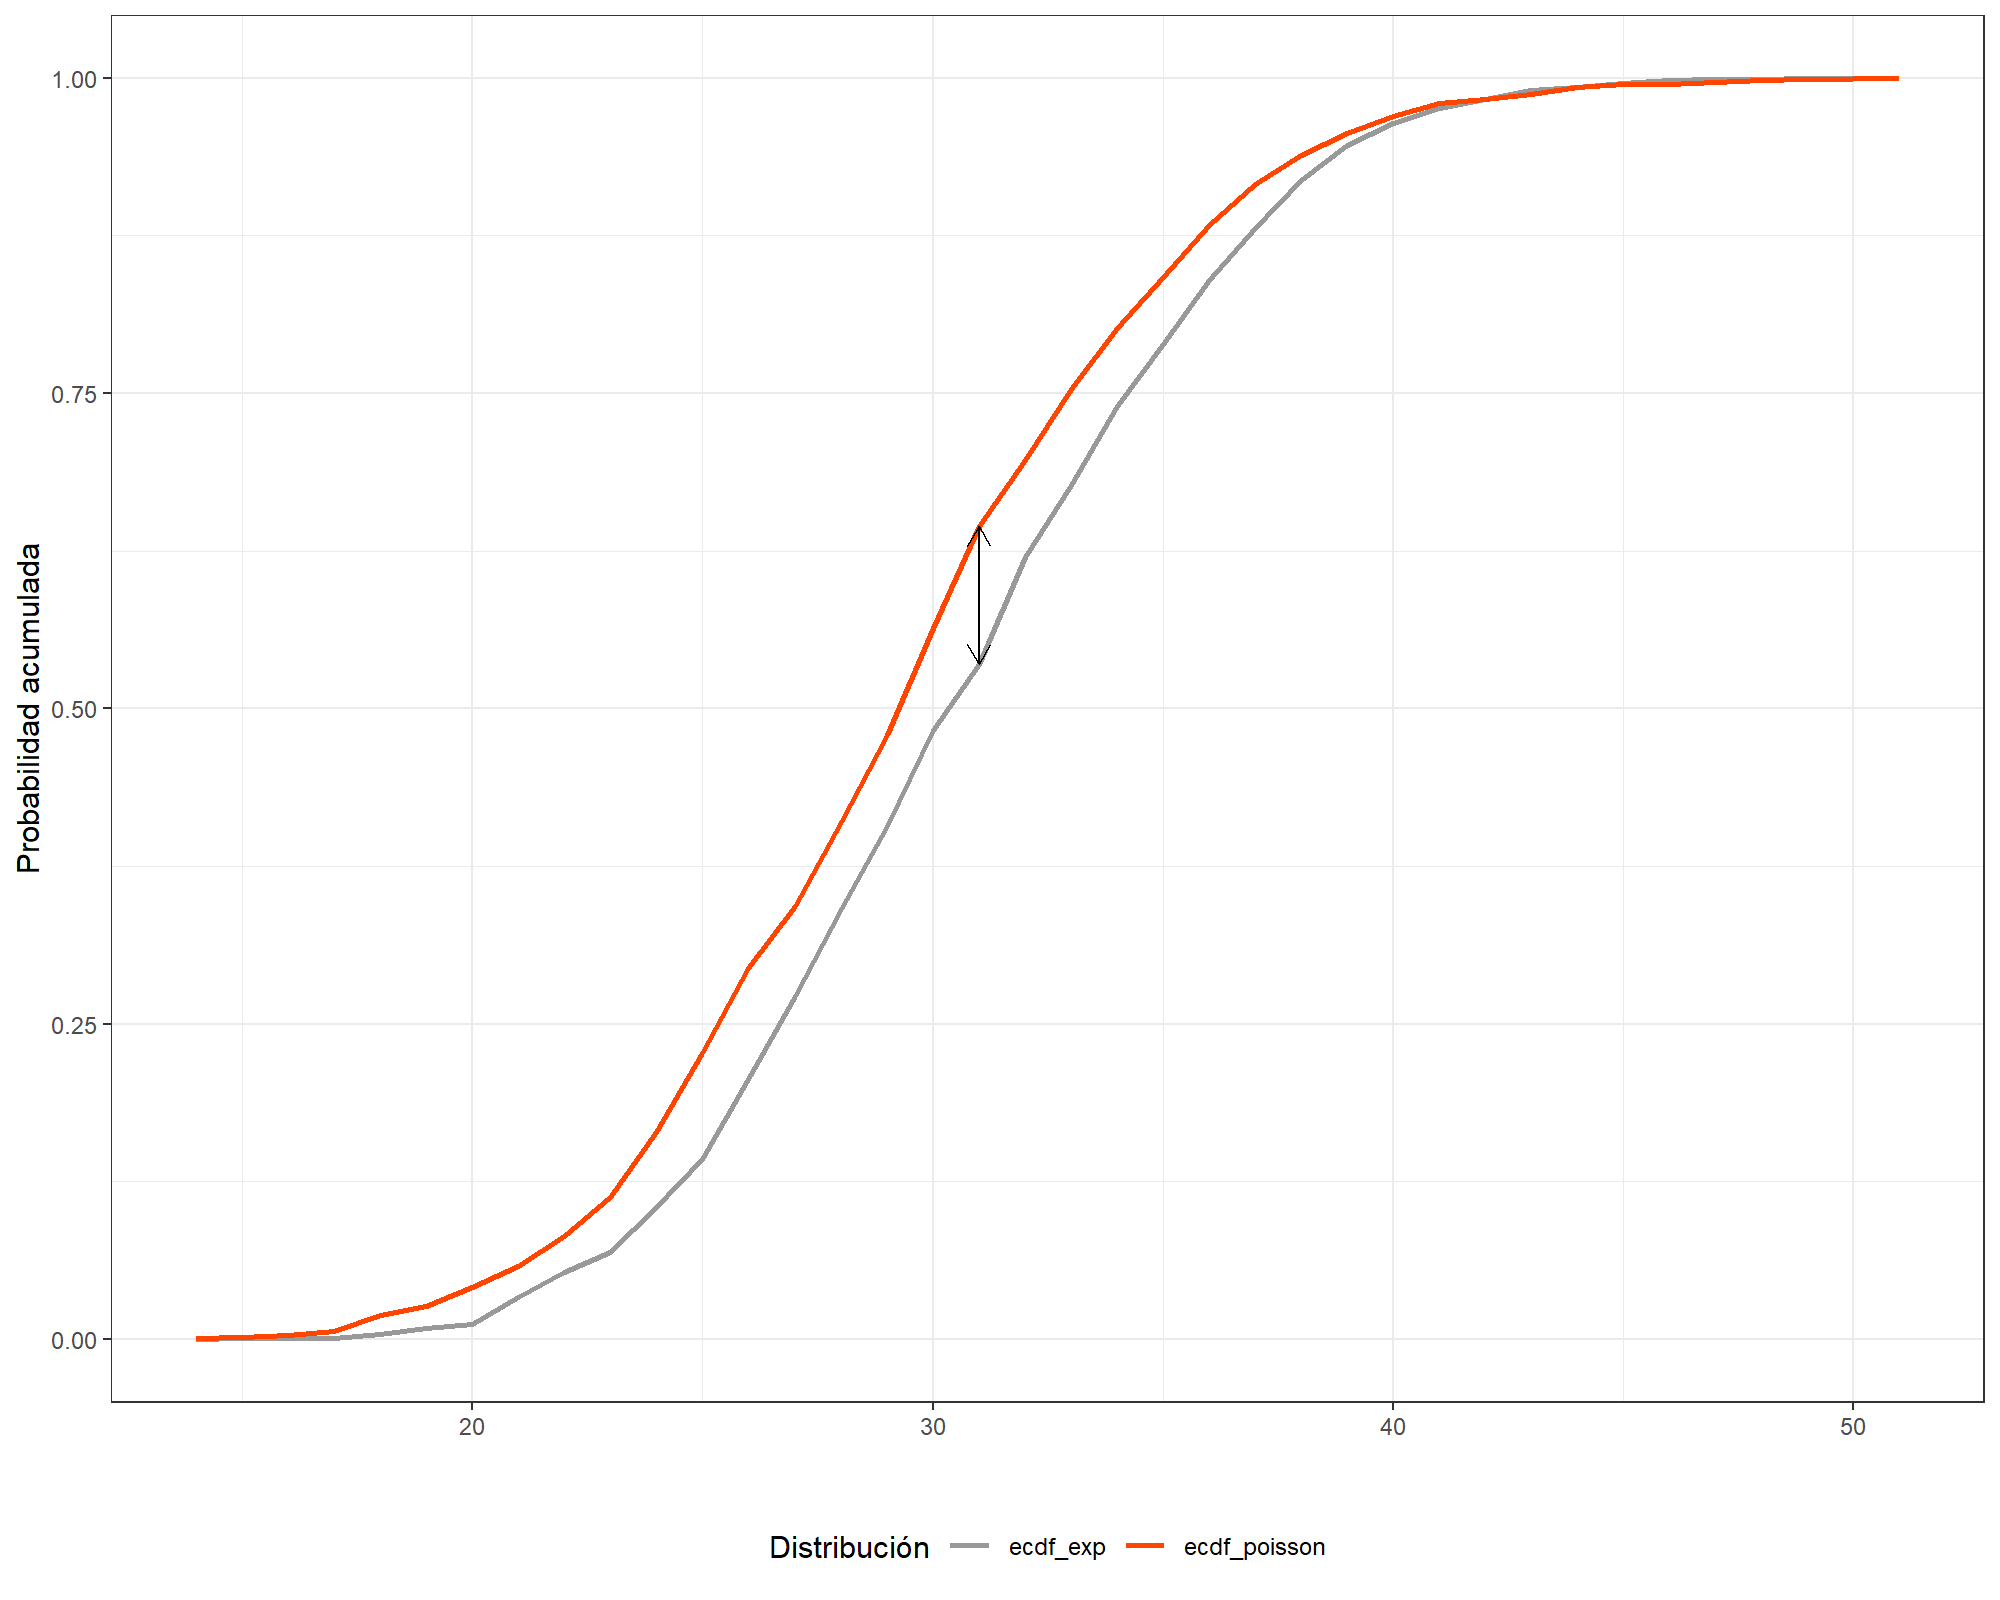
\includegraphics[scale=0.6]{figuras/distanciaKolmPE.png}
\caption{Distancia de Kolmogorov–--Smirnov entre ambas poblaciones}
\label{fig:3}
\end{figure}
\end{center}
 Para concluir si ambas poblaciones viene de una misma distribución se procede a aplicar la prueba de Cucconi, que es una prueba no paramétrica para comparar conjuntamente la tendencia central y la variabilidad (detectando cambios de ubicación y escala) en dos muestras. Lo s resultados son para el estadístico $C = 12.287$ y $p-valor = 0$, se rechaza la hipótesis nula que ambas poblaciones viene de una misma distribución.

\subsection{Aproximación mediante el uso de variables aleatorias Exponenciales}

Para reducir los cálculos, se reformula el método que utiliza variables aleatorias exponenciales, por el productos de variables aleatorias uniformes, debido a identidades logarítmicas. Se usan variables aleatorias uniformes estándar $U_{1}, U_{2},...U_{n}$ y N es el número entero más pequeño tal que: 

 \begin{equation}
    \prod_{k=1}^{n}U_{k} >e^{-\lambda} 
\end{equation}
Entonces N es Poisson $(\lambda)$, Lema 3.3 Capítulo 10 \cite{expvar} 

A continuación realizaremos una comparación entre las variables aleatorias de Poisson creadas a partir de la suma del producto de variables aleatorias uniformes y las creadas a partir de la biblioteca \textit{rpois}.

En la figura \ref{fig:4} de la página \pageref{fig:4} se muestra los histogramas de las dos poblaciones simuladas. En la figura \ref{fig:5} de la página \pageref{fig:5}, se muestran superpuestos los diagramas de densidad de ambas poblaciones 

\begin{center}
\begin{figure}
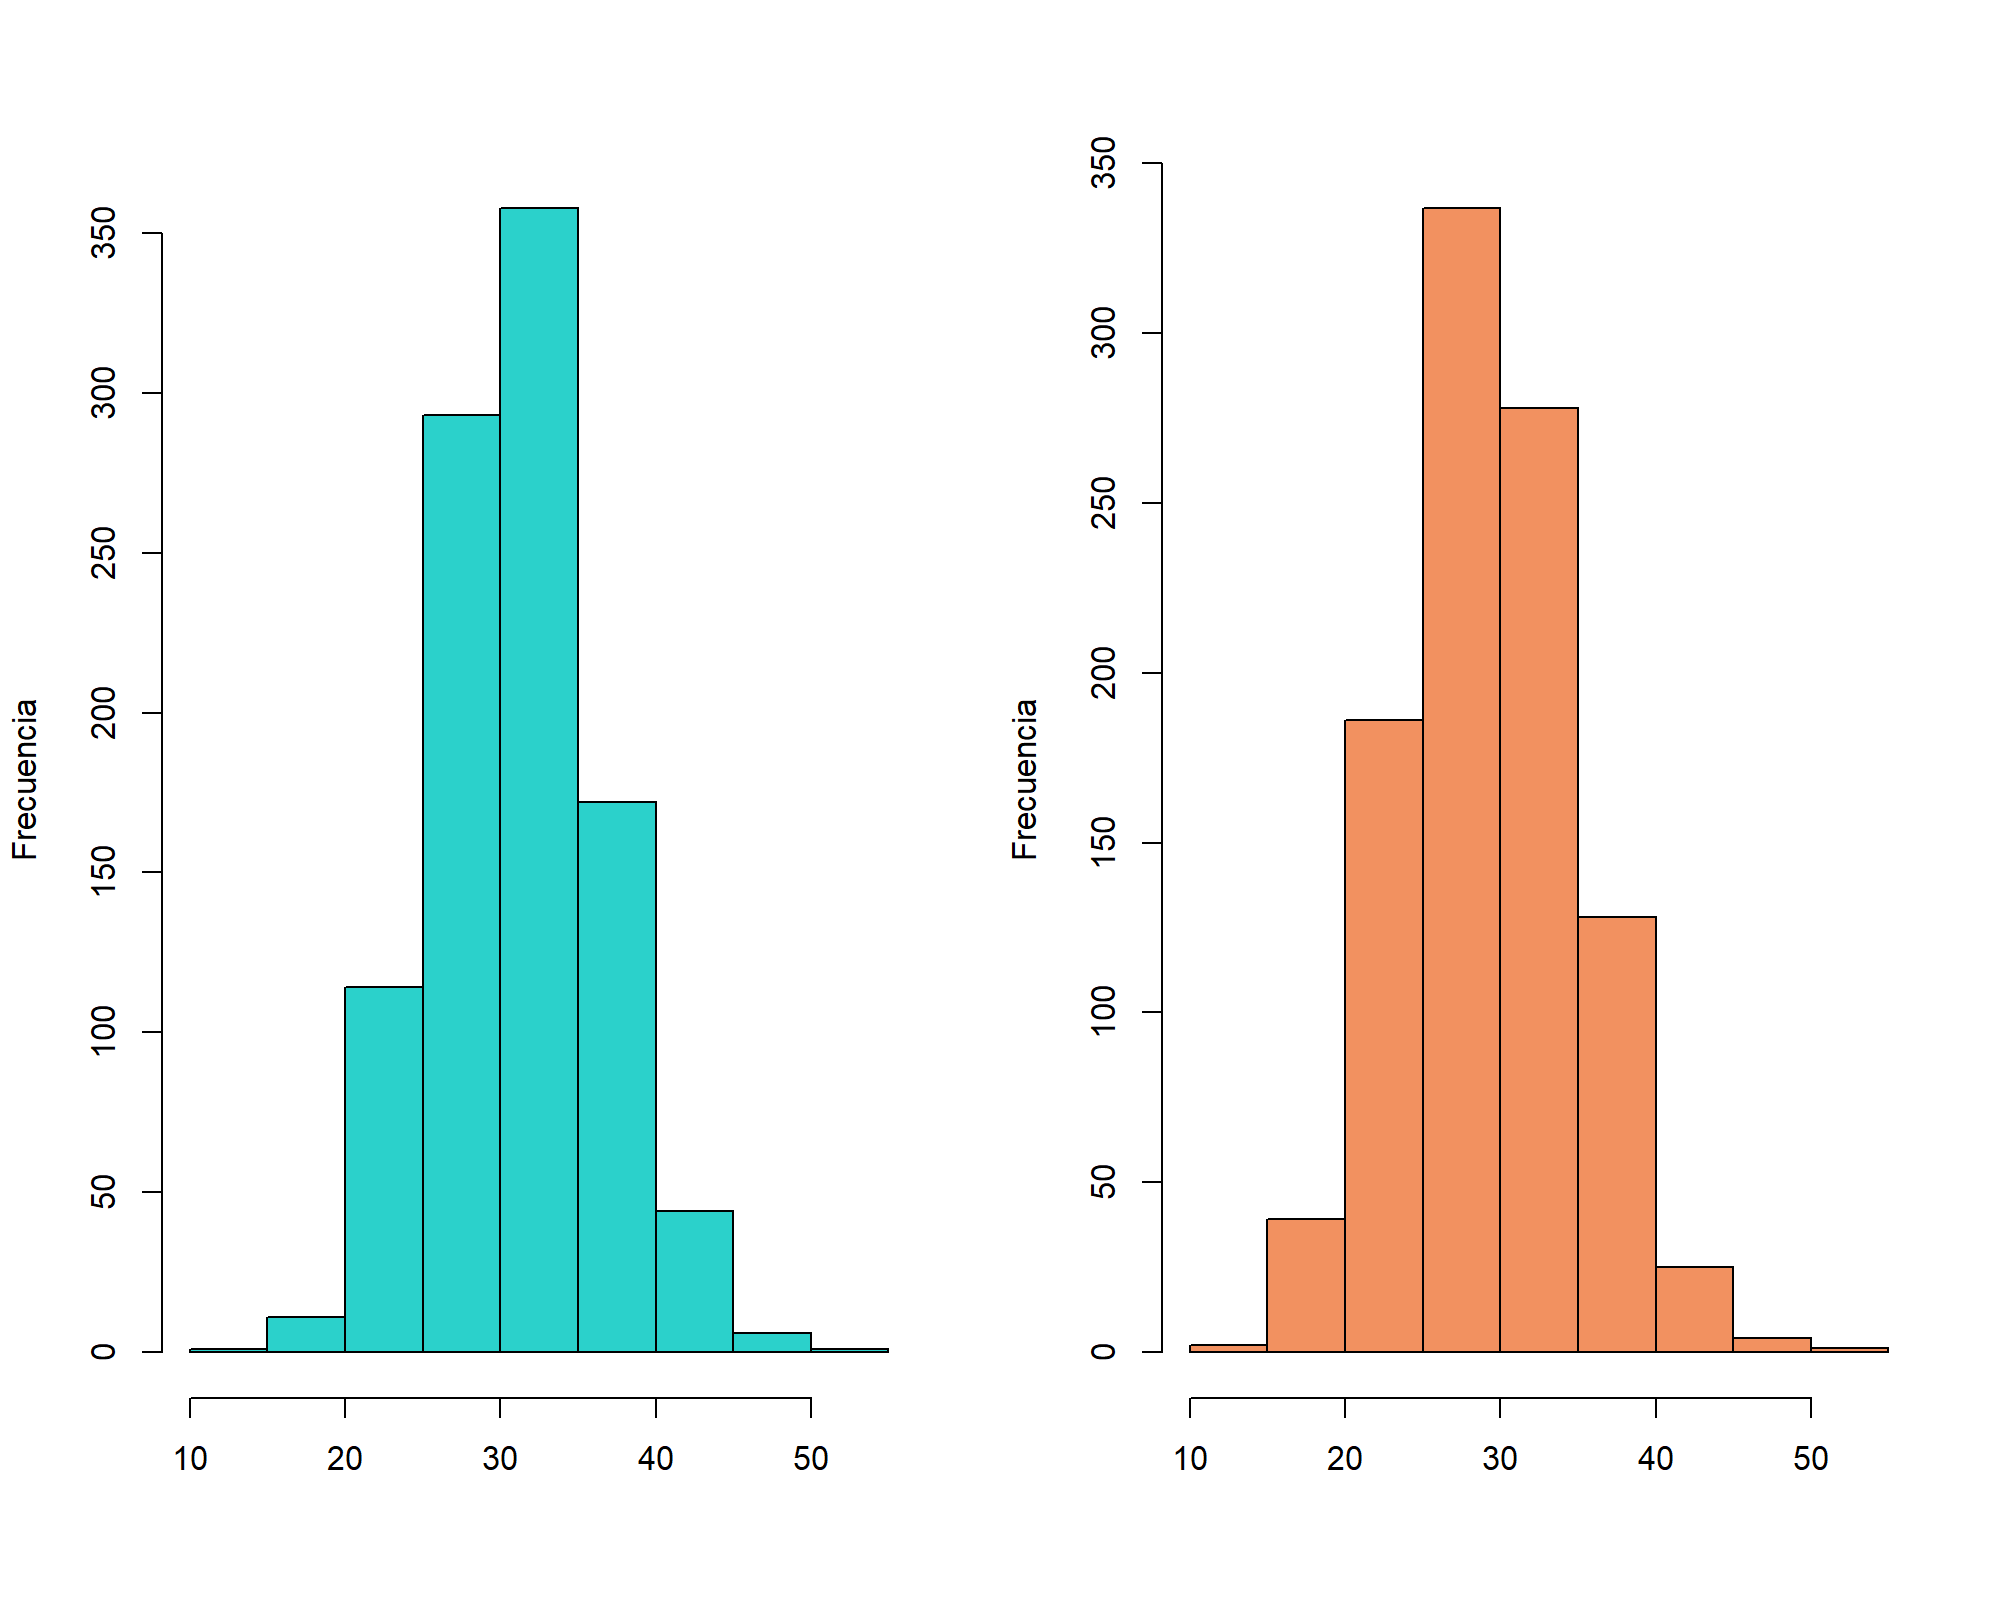
\includegraphics[scale=0.65]{figuras/AproxU2301.png}
\caption{Histogramas de las poblaciones simuladas, a la izquierda la aproximación a partir de la Uniforme y a la derecha la creada a partir de la biblioteca \textit{rpois}}
\label{fig:4}
\end{figure}
\end{center}

\begin{center}
\begin{figure}
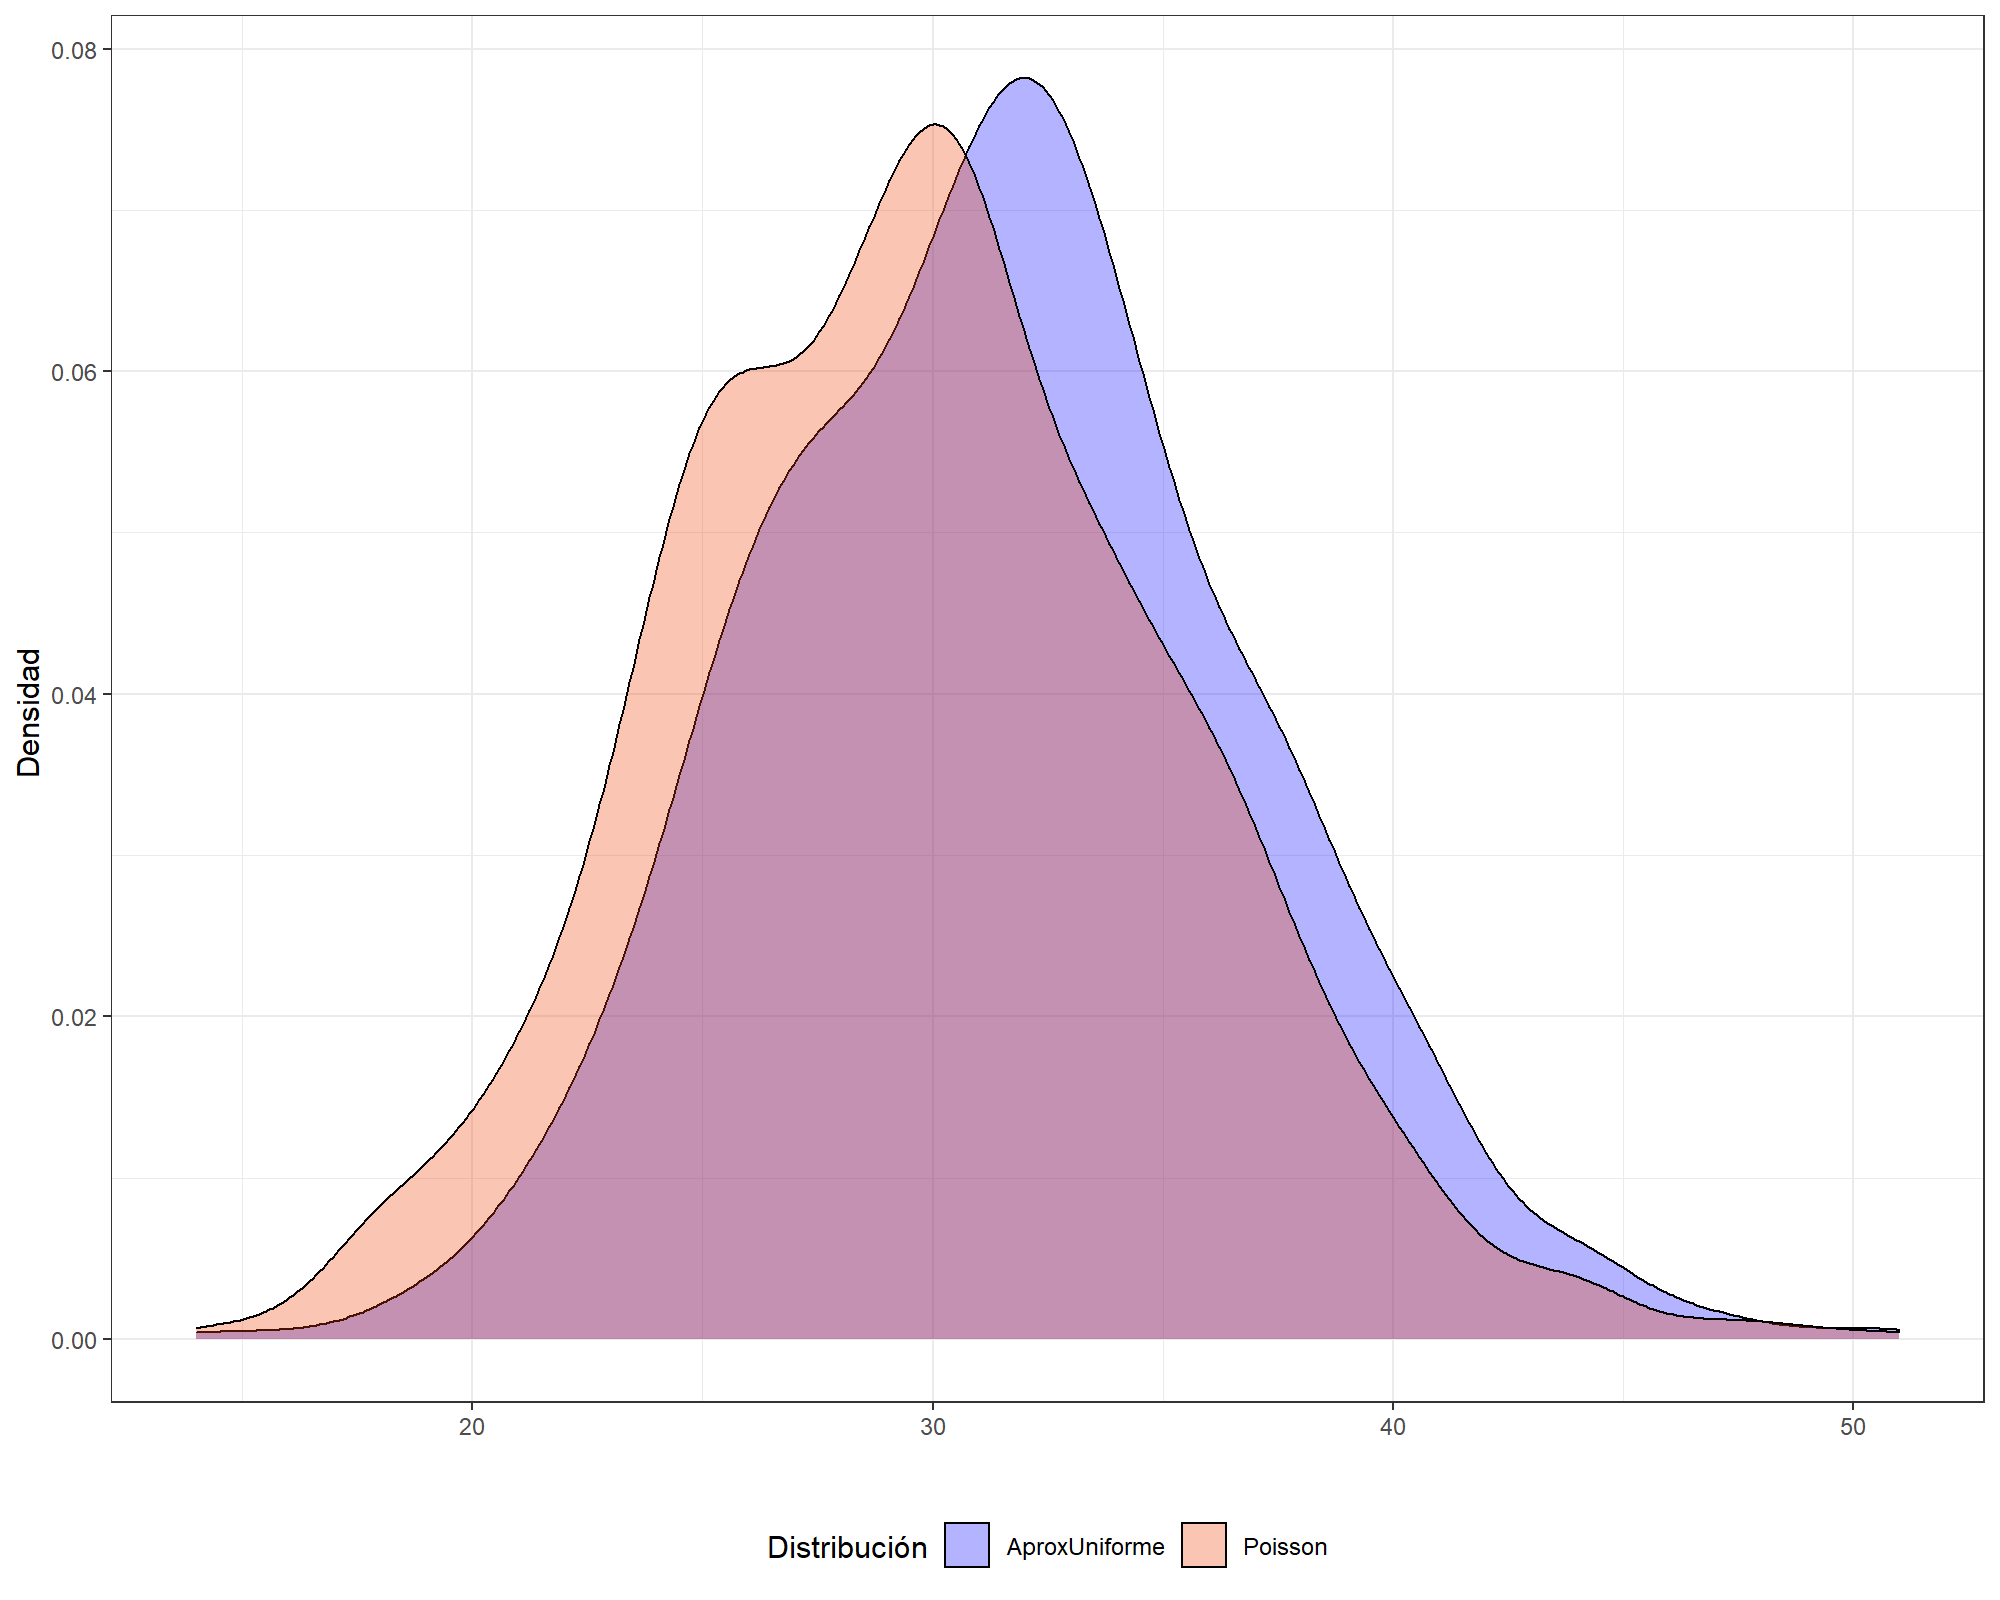
\includegraphics[scale=0.6]{figuras/densidadPU.png}
\caption{Diagramas de densidad de ambas poblaciones}
\label{fig:5}
\end{figure}
\end{center}
Para calcular la diferencia entre las distribuciones se realiza el cálculo de la distancia Kolmogorov–--Smirnov, que se define como la distancia vertical máxima entre las funciones de distribución acumulada empíricas de dos muestras, donde el valor de la distancia es $0.154$. Esto se puede observar en la figura \ref{fig:6} de la página \pageref{fig:6}.

\begin{center}
\begin{figure}
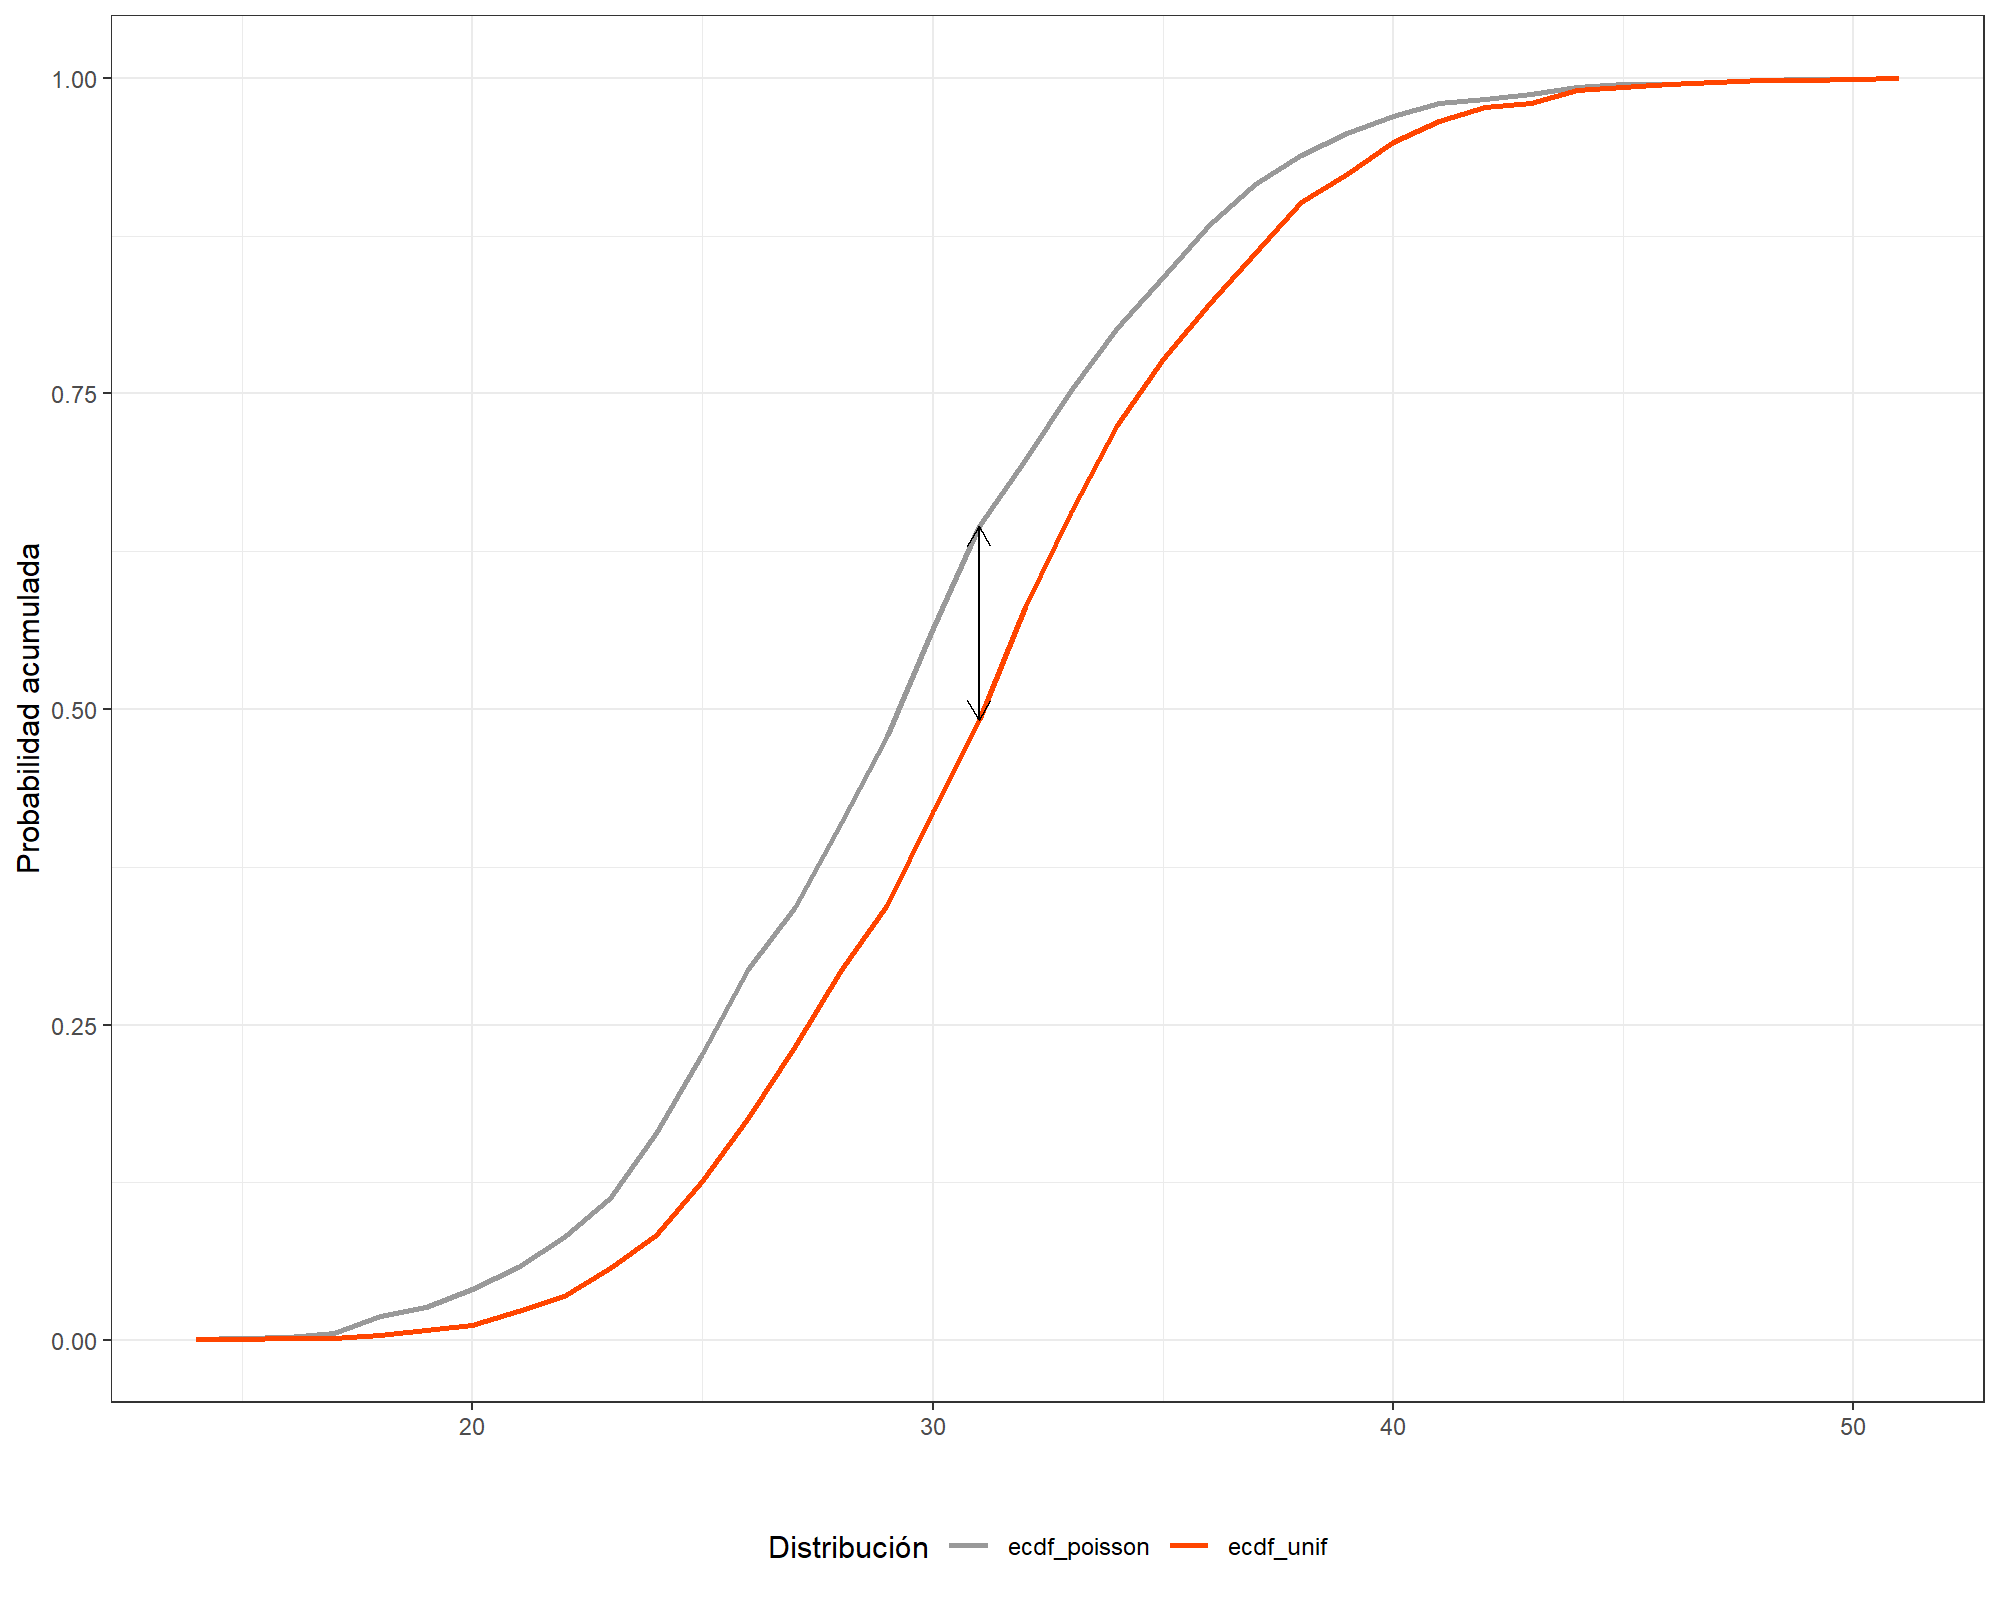
\includegraphics[scale=0.6]{figuras/distanciaKolmPU.png}
\caption{Distancia de Kolmogorov–--Smirnov entre ambas poblaciones}
\label{fig:6}
\end{figure}
\end{center}
 Para concluir si ambas poblaciones viene de una misma distribución se procede a aplicar la prueba de Cucconi, que es una prueba no paramétrica para comparar conjuntamente la tendencia central y la variabilidad (detectando cambios de ubicación y escala) en dos muestras. Lo s resultados son para el estadístico $C = 12.287$ y $p-valor = 0$, se rechaza la hipótesis nula que ambas poblaciones viene de una misma distribución.


El código general se encuentra disponible en el repositorio \href{https://github.com/Albertomnoa/Tareas_MPA/tree/master/Tarea3}{https://github.com/Albertomnoa/Tareas} 

\newpage
\bibliographystyle{plain}
\bibliography{Biblio}

\end{document}
